\documentclass[15pt]{article}
\linespread{1.6}
\renewcommand{\normalsize}{\fontsize{12pt}{10}\selectfont}  
\setlength{\parindent}{0pt}

% Packages
\usepackage[utf8]{inputenc}
\usepackage{multicol}
\usepackage{geometry}
\usepackage{times}
\usepackage{graphicx}
\usepackage{xcolor}
\usepackage{hyperref}
\usepackage{fancyhdr}
\usepackage{setspace}
\usepackage{titlesec}
\usepackage{caption}
\usepackage{hyperref}
\usepackage{rotating}
\usepackage{tabularx}
\usepackage{arabtex}
\usepackage{utf8}
\usepackage{float}
\usepackage[bottom]{footmisc}
\usepackage[justification=raggedright,
            singlelinecheck=false,
            format=plain,
            labelfont={bf,it},
            textfont=it]{caption}
\usepackage[
    backend=biber,
    style=ieee,
    sorting=ynt
    ]{biblatex}
    
\addbibresource{export.bib}
\setcode{utf8}
\title{College of Computer and Information Sciences}
\author{Mais Alharaki}

% Turn on the style
\pagestyle{fancy}
% Clear the header and footer
\fancyfoot{}
% Set the right side of the footer to be the page number
\fancyhf{}
\fancyhead[R]{Page \thepage\hspace{1pt} of~\pageref{lastpage}}
\pagestyle{fancy}

% Adjust section title spacing
\titlespacing*{\section}{0pt}{0.2\baselineskip}{0.3\baselineskip}
\titlespacing*{\subsection}{0pt}{0\baselineskip}{0\baselineskip}
\titlespacing*{\subsubsection}{0pt}{0.1\baselineskip}{0.1\baselineskip}

\geometry{a4paper, margin=1in}
\setlength{\parskip}{\baselineskip}%

\begin{document}

\begin{titlepage}
    
    \begin{figure*}[ht!]
        \centering
        
\includegraphics[height=2cm]{2023.jpg}
        \hspace{4cm}
        
\includegraphics[height=2cm]{pnu.jpg}
    \end{figure*}
    \vspace{.5cm}
    \centering
    {\textcolor{gray}{College of Computer and Information Sciences} \par}

    \vfill

    \centering
    {\LARGE\bfseries Research Project Report\par}
    \vspace{.5cm}
    {\large Master of Science in Computing (Data Science)\par}
    \vfill
    \begin{singlespace}
    \setstretch{1.2}
    \LARGE
    A Deep Learning Approach to Arabic Reverse Dictionary
    \end{singlespace}
    \vspace{2cm}

    \vfill
    
    \begin{center}
    \renewcommand{\arraystretch}{1.5}
    \begin{tabular}{|l|l|}
        \hline
        \textbf{Student Name} & {Mais Alharaki} \\
        \hline
        \textbf{Student ID} & 444010562 \\ 
        \hline
        \textbf{Submission Date} & 2 May 2024 \\ 
        \hline
    \end{tabular}
    \end{center}

    \vfill
    
    Second Semester 2023--2024
\end{titlepage}

\begin{spacing}{-2}
\tableofcontents 
\end{spacing}

\newpage

\section*{Declaration}

\noindent
\textbf{I hereby certify that:}

\begin{itemize}
\item[-] This material, which I now submit for assessment on the programme of study leading to the award of MSc Computing (Data Science) is entirely my own work, and that I have exercised reasonable care to ensure that the work is original, and does not to the best of my knowledge breach any law of copyright, and has not been taken from the work of others save and to the extent that such work has been cited and acknowledged within the text of my work.
\item[-] Due acknowledgement has been given in the bibliography and references to ALL sources be they printed, electronic or personal.
\item[-] Unless this dissertation has been confirmed as confidential, I agree to an entire electronic copy or sections of the dissertation to be available to allow future students the opportunity to see examples of past dissertations.
\item[-] I agree to my dissertation being submitted to a plagiarism detection service, where it will be stored in a database and compared against work submitted from this or any other Department or from other institutions using the service. In the event of the service detecting a high degree of similarity between content within the service this will be reported back to my supervisor and program leader, who may decide to undertake further investigation that may ultimately lead to disciplinary actions, should instances of plagiarism be detected.
\item[-] I have read the PNU Policy Statement on Ethics in Research (\url{https://www.pnu.edu.sa/ar/Deanship/PostGraduate/Documents/دليل%20الأخلاقيات%20البحثية%20والأمانة%20العلمية%20والملكية%20الفكرية.pdf}) and I confirm that ethical issues have been considered, evaluated and appropriately addressed in this research.
\end{itemize}

\vspace{1cm}

\noindent
Signed:

\noindent
Candidate Name: \underline{Mais Alheraki}

\noindent
ID Number: \underline{444010562}

\noindent
Date: \underline{2 May 2024}



\newpage

\thispagestyle{empty}
\listoffigures
\newpage
\thispagestyle{empty}
\listoftables
\newpage

\section*{List of abbreviations}
\begin{enumerate}
    \item[] RD: Reversed Dictionary
    \item[] NLP: Natural Language Processing
    \item[] NLG: Natural Language Generation
    \item[] NLU: Natural Language Understanding
    \item[] BERT: Bidirectional Encoder Representations from Transformers
    \item[] Seq2Seq: Sequence to Sequence
\end{enumerate}
\newpage

\section*{Abstract}

The domain of reverse dictionaries, while advancing in languages like English and Chinese, remains significantly underdeveloped for less resourced languages, such as Arabic. This study attempts to explore a data-driven approach to enhance word retrieval processes in Arabic reverse dictionaries. The research focuses on the ArabicNLP 2024 Shared Task, which provides a dataset of 39,214 word-gloss pairs, each with a corresponding target word embedding. The proposed solution aims to surpass the baseline performance by employing state-of-the-art deep learning models and innovative data augmentation techniques. The methodology involves enriching the dataset with contextually relevant examples, training a T5 model for word embedding prediction, and evaluating the results using Mean Squared Error and Cosine similarity. The study aims to contribute to the advancement of Arabic reverse dictionaries.

\newpage

\section{Introduction}

While reversed dictionaries have witnessed advancements in languages like English and Chinese (e.g., WantWords \cite{Qi2020}), their development for Arabic remains significantly underdeveloped. This gap is particularly concerning for a language with a rich linguistic heritage and widespread use. Despite this, robust and technologically advanced tools for reverse lexical searches in Arabic are scarce, with the only ongoing effort being the 1st Arabic Reverse Dictionary shared task launched in 2023 by the King Salman Global Academy for Arabic Language \footnote{\url{https://arai.ksaa.gov.sa/sharedTask/}}.


\subsection{Content of study}

This research aims to address the limitations of existing Arabic reverse dictionary models by proposing a data-driven approach that leverages deep learning techniques to enhance word retrieval processes. We focus on the ArabicNLP 2024 Shared Task dataset, which provides a rich collection of approximately 39k word-gloss pairs extracted from various Arabic dictionaries, each associated with a corresponding target word embedding. The proposed solution employs state-of-the-art deep learning models and innovative data augmentation techniques to improve performance.

\subsection{Problem Statement \& Motivation}

The Arabic language, with its intricate morphology and diverse dialects, presents unique challenges for Natural Language Processing (NLP) tasks. Reverse dictionaries are crucial tools for language learners, translators, and researchers, enabling them to identify words based on their meanings or descriptions.

However, existing Arabic reverse dictionary models are often limited in scope and functionality, frequently relying on traditional dictionary structures that fail to capture the nuances and complexities of the language. This research is motivated by the desire to enrich this field by exploring new methodologies that can significantly enhance the performance of Arabic reverse dictionaries.


\subsection{Aim and objectives}

This project aims to enhance word retrieval processes in Arabic by leveraging data-driven techniques to establish a more intuitive and accurate connection between conceptual descriptions and corresponding terms. This approach is specifically designed to improve the language learning experience by utilizing sophisticated data analytics to map natural language inputs to lexical outputs. Focusing on Arabic, a less explored language in this domain, presents a unique opportunity to contribute significantly to the field of data science by extending its applications to new linguistic territories.

\subsection{Proposed solution}

This research leverages the new ArabicNLP 2024 Shared Task dataset, comprising 39,214 word-gloss pairs with corresponding target word embeddings. Our goal is to surpass the baseline performance by employing cutting-edge deep learning models and innovative data augmentation techniques. Figure \ref{fig:rd-flow} illustrates the proposed solution's workflow.

\begin{figure}
    \centering
    \captionsetup{justification=centering}
    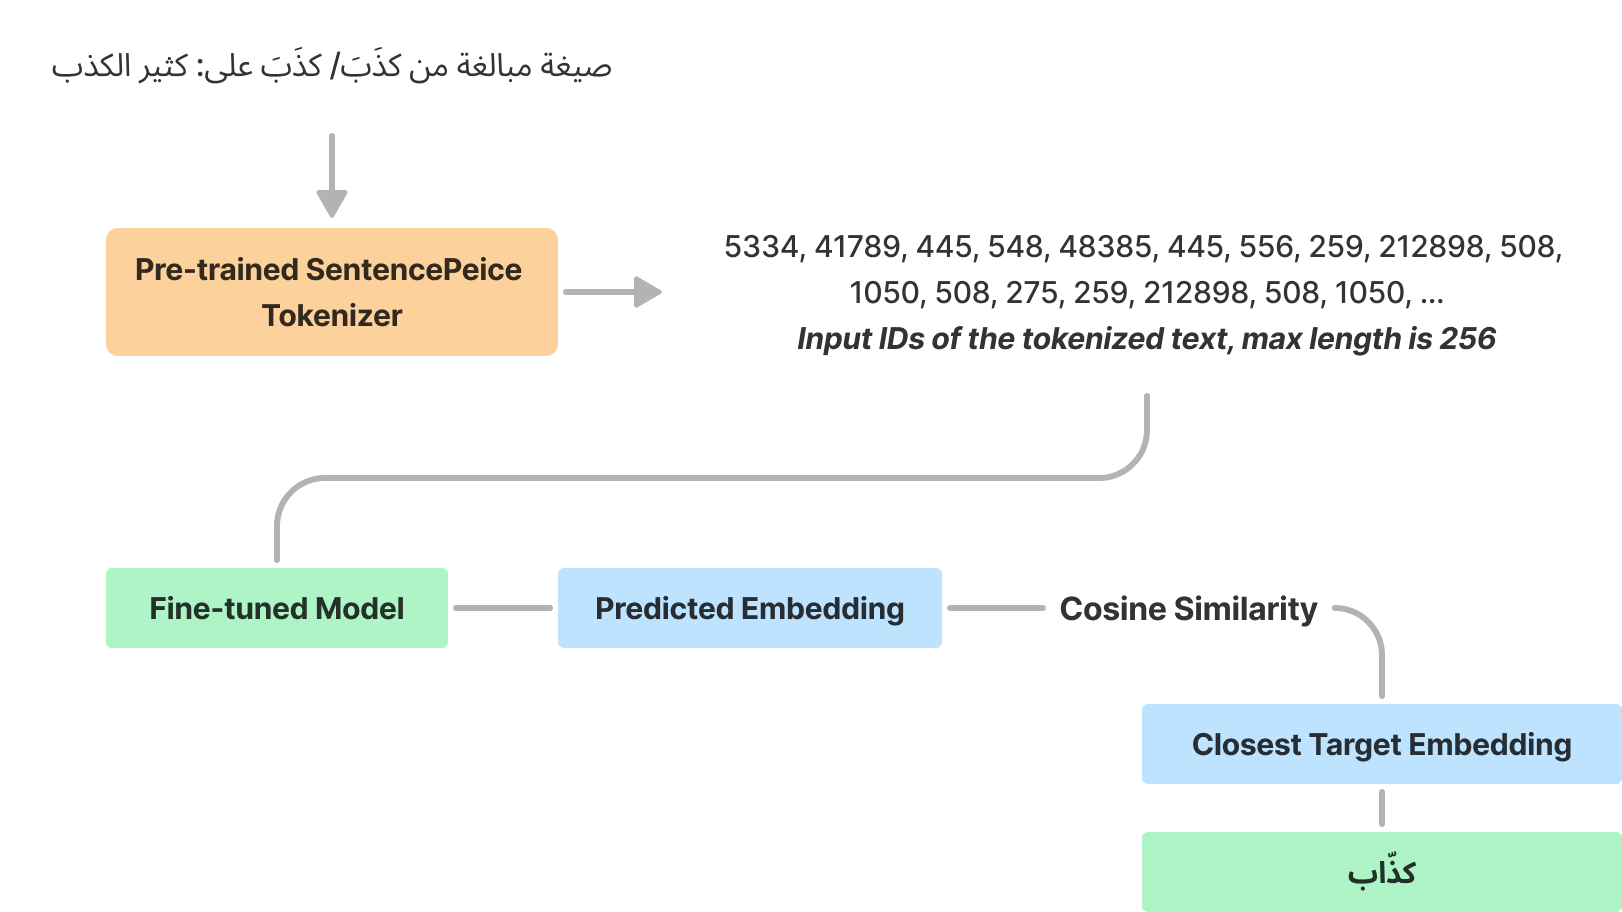
\includegraphics[width=\textwidth]{rd-flow.png}
    \caption{The workflow of a reverse dictionary}
    \label{fig:rd-flow}
\end{figure}

The proposed solution is twofold:

\begin{enumerate}
    \item \textbf{Data Enrichment:} The dataset will be enriched with contextually relevant examples to enhance the model's understanding of word meanings. This will be achieved by leveraging a large Arabic text corpus to curate examples for each word-gloss pair.
    \item \textbf{T5 Model Integration:} A T5 model will be trained to predict word embeddings from the enriched dataset.
\end{enumerate}

\newpage

\subsection{Structure of the report}

The upcoming sections are structured as follows:

\begin{enumerate}
    \item Section 2 provides background material on natural language processing, deep learning, and reverse dictionaries.
    \item Section 3 reviews related work in the field of reverse dictionaries, highlighting recent advancements and research gaps.
    \item Section 4 outlines the methodology and proposed solution, detailing the dataset, data expansion techniques, model architecture, and evaluation metrics.
    \item Section 5 presents the results of the experiments and discusses the findings.
\end{enumerate}

\newpage

\section{Background material}

This chapter lays the groundwork for understanding the subsequent sections of this report by exploring the fundamentals of natural language processing, deep learning, text embeddings, transformers, and more. These disciplines are instrumental to the overall research presented here.

\subsection{Natural Language Processing}

Language is the way we communicate and exchange information, it’s composed of symbols, rules and repetitive expressions. Natural Language Processing or NLP is a field where AI and linguistics cross together. It's interested in enabling machines to understand and model language, therefore enabling more natural communication between humans and machines.

NLP encompasses two major subfields: Natural Language Understanding (NLU) and Natural Language Generation (NLG). NLU focuses on enabling computers to comprehend the meaning of words, phrases, and expressions within human language. In contrast, NLG concerns the process of generating meaningful phrases and paragraphs, essentially allowing machines to "write" human-like text \cite{Khurana2023}.

\subsection{Deep learning}

Deep learning is a subfield of machine learning inspired by the structure and function of the human brain. It utilizes artificial neural networks (ANNs) with multiple hidden layers, enabling the extraction of complex patterns from large amounts of data. This capability has revolutionized various fields, including computer vision, natural language processing (NLP), and speech recognition.

Though the idea can be traced back many years, deep learning only recently has proved to outperform traditional ML algorithms in many areas, including NLP. In 2016, \cite{Vaswani2017} introduced the Transformer architecture, which has since become the foundation for many state-of-the-art NLP models, such as BERT, GPT-3, and T5.

However, training deep learning models from scratch often requires significant computational resources and large amounts of labeled data. This can be a barrier for tasks with limited data availability. Here's where transfer learning comes in as a powerful technique.

\subsubsection{Transfer Learning}

Transfer learning is an approach that leverages knowledge gained from a pre-trained deep learning model on a source task and applies it to a new, related target task. By transferring the learned weights and features from a pre-trained model, a target model can achieve good performance even with limited training data. This is particularly beneficial for NLP tasks, where obtaining large amounts of labeled data can be expensive and time-consuming.

A popular example of transfer learning models borrowd from the computer vision field is the ImageNet \cite{ILSVRC15} dataset, where models trained on it can be used for other image classification tasks, naming VGG \cite{Simonyan2014}, ResNet \cite{He2015}, and Inception \cite{Simonyan2014}.

Models trained on large corupses of text are known as "language models", these models learn to assign probabilities to tokens (words or characters) given their occurance in the training corpus. Pre-trained language models can be used as a starting point, or as sometimes referred to as \textbf{checkpoints}, to a lot of downstream NLP tasks such as sentiment analysis, text classification, and topic modeling, instead of starting from scratch, which saves a vast amount of time and computational resources, given that a model have already learned the patterns from the original data.

Neural networks allowed for the development of more complex language models, where models can analyzed huge amounts of text data and learn the patterns and relationships between words, using various architectures such as RNNs, LSTMs, and Transformers.

\subsubsection{Sequence to Sequence approach for language modeling}

The sequence to sequence (Seq2Seq) approach is a powerful deep learning architecture specifically designed for tasks that involve processing and generating sequences. In NLP, this translates to tasks like machine translation, where an input sequence in one language is transformed into an output sequence in another language. Seq2Seq models typically consist of two deep neural networks:
\begin{enumerate}
    \item[-] Encoder: This network processes the input sequence and encodes it into a fixed-length vector representation capturing the semantic meaning.
    \item[-] Decoder: This network utilizes the encoded representation from the encoder and generates the output sequence one element at a time, conditioned on the previously generated elements.
\end{enumerate}

\subsubsection{Tokenization and text embeddings}

Tokenization is the process of breaking down text data into smaller units suitable for processing by deep learning models. These units can be words, characters, or even sub-word units like morphemes. The choice of tokenization strategy can significantly impact the performance of deep learning models in NLP tasks.

Text embeddings represent the tokens as numerical vectors in a high-dimensional space, where words with similar meanings tend to be positioned closer together. Popular techniques for text embedding include Word2Vec and GloVe, which learn these representations by analyzing large text corpora.

In the case of deep learning models, text embeddings are often learned as part of the training process, and is often the result of the encoder part of a sequence-to-sequence model, where the input text is transformed into a fixed-length vector representation.

\subsubsection{SentencePiece tokenizer}

SentencePiece is an unsupervised text tokenizer, used by the T5 models for text data processing \cite{Kudo2018}. Unlike traditional word-based tokenization, SentencePiece utilizes subword units, which are smaller linguistic components like prefixes, suffixes, and morphemes. This approach offers several advantages. Firstly, it allows T5 to effectively handle OOV words by combining subword units to represent them. Secondly, SentencePiece is language-independent, enabling T5 to process text in diverse languages with a single tokenizer.

During tokenization, SentencePiece analyzes the training corpus to identify frequently occurring subword units and builds a vocabulary. When processing text, it segments the input into these subword units and assigns them unique token IDs, which the T5 model uses for its internal operations. This subword-level representation provides T5 with a more granular understanding of the text, enhancing its ability to perform various NLP tasks effectively.

\subsubsection{Transformer architecture: a paradigm shift}

The Transformer architecture, introduced by Vaswani et al. in 2017 in the famous paper “Attention is All You Need” \cite{Vaswani2017}, has become a dominant force in NLP due to its ability to efficiently capture long-range dependencies within sequences. Unlike RNNs, which process sequences sequentially, Transformers rely solely on attention mechanisms. These mechanisms allow each element in the input sequence to attend to (focus on) other elements, enabling the model to understand the context of each word in relation to the entire sequence. This parallel processing approach facilitates faster training compared to RNNs and is particularly effective for tasks requiring long-range dependency modeling, such as machine translation and text summarization.

\subsubsection{Pre-trained transformer models: BERT and T5}

While the core Transformer architecture provides a powerful foundation, further advancements have led to the development of specialized pre-trained models like BERT and T5. These models leverage the strengths of Transformers and are pre-trained on massive amounts of unlabeled text data, allowing them to learn general contextual representations of language.

\begin{enumerate}
    \item[-] \textbf{BERT (Bidirectional Encoder Representations from Transformers)}: Introduced by Google AI \cite{devlin2018} in 2018, BERT is a pre-trained Transformer model that excels at understanding the context of words in a sentence and their relationships. It can be fine-tuned for various NLP tasks like question answering and sentiment analysis. However, BERT requires fine-tuning for specific tasks, which can be computationally expensive.
    \item[-] \textbf{T5 (Text-to-Text Transfer Transformer)}: Introduced also by Google AI in 2019 \cite{Raffel2019}, T5 utilizes a text-to-text format for all NLP tasks. It employs a single encoder-decoder architecture and learns to transform the input sequence into the desired output sequence. This approach makes T5 versatile, allowing it to handle a wide range of tasks by simply changing the format of the input and desired output. T5 often requires less fine-tuning compared to BERT, making it quicker to deploy for various tasks. However, it might not achieve the same level of deep contextual understanding as BERT in tasks where this is crucial.
\end{enumerate}

\subsection{Reverse dictionaries}

Dictionaries in their conventional form map words to a set of meanings or definitions, often combining them with some examples on how the words are used in context. Dictionaries are the foundation of various NLP tasks, serving as lexical resources, where they help in understanding information such as word meanings, parts of speech, and relationships between words. Tasks such as stemming and lemmatization also rely on dictionaries to return words to their base form. However, traditional dictionaries are unidirectional, providing word meanings based on the input word.

Reverse dictionaries are a form of dictionaries where a description yields a set of words from the dictionary that semantically matches the description. Traditionally used as tools for linguistic exploration, reverse dictionaries have evolved to play a significant role in data science. A prime use-case is their application in data exploration and analysis, where reverse dictionaries facilitate the identification of relevant features within complex textual datasets by generating key terms or phrases. This enhances the efficiency of data mining and fosters the discovery of new insights \cite{Chen2022}.

In machine learning, reverse dictionaries aid in feature engineering, enriching model inputs with nuanced context. This utility extends to automated metadata generation for effective data cataloging and management. Additionally, they enhance content curation and recommendation systems, offering more precise content descriptors and improving recommendation relevance.

Furthermore, reverse dictionaries streamline text summarization and topic modeling \cite{Griffiths2004}, assisting in distilling essential information from large text volumes. They also play a crucial role in improving chatbot and customer service automation by accurately interpreting user queries and intents.

\subsection{ArabicNLP 2024 Shared Task}

The KSAA-CAD Shared Task\footnote{The new task has been launched in May this year, more information can be found here: \href{https://arai.ksaa.gov.sa/sharedTask2024/}{arai.ksaa.gov.sa/sharedTask}} is a part of the ArabicNLP \footnote{\href{https://arabicnlp2024.sigarab.org/}{arabicnlp2024.sigarab.org}} conference for 2024, and it aims to advance the field of Arabic natural language processing by providing a platform for researchers to collaborate and innovate. 

This task specifically targets the development of reverse dictionary models capable of predicting words from their definitions in Arabic. Participants are provided with a dataset containing 39k instances, and consisting of word-gloss pairs and corresponding word embeddings, challenging them to build models that can accurately predict the target words based on the provided glosses.

We particpated in this task, and the proposed solution is based on the dataset provided by the organizers. The aim is to ourperform the baseline, and generate new features on the given dataset. Our solution will be submitted to the shared task for evaluation, and a system design paper will be submitted to the conference, based on this report.

\newpage

\section{Related work}

Understanding the meaning behind words, even within the same language, presents a significant challenge for machines. Monolingual reversed dictionaries address this directly, aiming to identify a target word based on its definition in the same language. This task is particularly crucial for languages like Arabic, with its rich vocabulary and unique cultural nuances. However, research in this area remains less explored compared to other languages with rich resources.

\subsection{Previous studies}

One notable recent contribution is the work presented by ElBakry et al \cite{Albakry2023}. (2023) as part of the ArabicNLP 2023 Shared Task, where they demonstrate an approach to Arabic reverse dictionary tasks, successfully handling both Arabic and English definition inputs. It utilizes an ensemble of fine-tuned BERT models, specifically CamelBERT-MSA and MARBERTv2, to predict word embeddings from provided definitions. By leveraging an ensemble strategy, the authors achieved improved results compared to single models, highlighting the benefits of this approach.

On the same task another attempt by Qaddoumi \cite{Qaddoumi2023}, a method is introduced to enhance Arabic word embeddings using a modified BERT Multilingual model with data augmentation, targeting improvements in Arabic reverse dictionary tasks. By customizing BERT for Arabic and employing data augmentation strategies, the study achieves significant enhancements in semantic accuracy. However, it suggests further exploration into the effects of data augmentation and the need for expanded datasets.

Building on this, Sibaee et al. \cite{Sibaee2023} presently employs a SemiDecoder architecture combined with an SBERT encoder. This methodology excels in encoding word definitions into vectors using SBERT, followed by training with the SemiDecoder model. The approach leverages SBERT's proficiency in capturing semantic similarity and the SemiDecoder's training efficiency, leading to a high ranking in the shared task.

Other languages received more research in the area of RDs. Mane et al. \cite{Mane2022} proposed a unique approach to reverse dictionaries with mT5, aiming at Indian languages support, where mT5 was employed for its ability to understand and generate language across multiple languages. It contrasts with BERT's Masked Language Modeling, focusing instead on translating and understanding user inputs to produce accurate word predictions. The results showed that mT5 outperformed BERT-based models in the reverse dictionary task for both Indian languages and an English baseline.

Ardoiz et al. \cite{Ardoiz2022}, in the SemEval RD task, studied the significance of high-quality lexicographic data in the efficiency of reversed dictionaries models. They suggest that refining the dataset by incorporating high-quality lexicographic data could significantly impact the task's outcomes, emphasizing the need for a robust dataset for optimal model performance. Their methodology involved a sentence-transformer model named “distiluse-base-multilingual-cased-v2”, which was trained to make the definition embeddings as similar as possible as the word gloss.
On the other hand, Tran et al. 2022 in SemEval RD task, evaluates Transformer-based models enhanced with LST and BiLSTM layers for reverse dictionary across five languages, named English, Italian, Spanish, French and Russian, showcasing partial improvements over the CODWOE (COmparing Dictionaries and WOrd Embeddings) competition's baseline. It explores monolingual, multilingual, and zero-shot cross-lingual settings, providing insights into the viability of cross-lingual methodologies.

Chen et al. 2022 \cite{Chen2022} took a different approach on the English language by embedding both the definitions and words into the same shared space using transformer-based architectures to optimize the model across both tasks simultaneously. The model demonstrated superior performance in reverse dictionary tasks, achieving high accuracy and consistency over previous methods. For definition modeling, while showing improvements, the results suggest areas for future enhancement, particularly in generating higher-quality definitions as indicated by human evaluations and BLEU scores.

Covering a specific instance of the English reversed dictionary, Siddique et al. 2022 \cite{Siddique2022} focused on adjective phrases in Precisiated Natural Language, as mentioned that adjectives count for a large amount of content in natural language, hence highlighting the importance of a better representation for it. The proposed transformer-based model was reported to outperform the Onelook.com and WantWords online reverse dictionaries.

Following similar approaches in literature, Yan et al. 2020 \cite{Yan2020} incorporated BERT and mBERT into the RD task for both monolingual and cross-lingual contexts. The authors propose a method that enables effective word prediction from descriptions without needing parallel corpora for cross-lingual tasks. This approach addresses challenges such as data sparsity, polysemy, and the alignment of cross-lingual word embeddings. The methodology involved modifying the input sequence to include masked tokens that BERT or mBERT would predict, converting these predictions into word scores, and using these scores to rank the possible target words.

Zhang et al. 2019 \cite{Zhang2019} presents a cross-lingual, multi-channel reverse dictionary model, addressing the variability of input queries and targeting both high and low-frequency words, showing state-of-the-art performance across English and Chinese datasets. The model combines a sentence encoder with multiple characteristic predictors (POS, morpheme, word category, sememe) to enhance word retrieval from descriptions. Experiments demonstrate significant improvements over conventional methods and commercial systems, particularly for human-written descriptions, while suggesting the model's adaptability to diverse linguistic features and robustness in handling variable inputs.

Finally, covering monolingual English RD, Pilehvar et al. 2019 \cite{Pilehvar2019} and Hedderich et al. 2019 \cite{Hedderich2019} emphasized on the importance of representing multi-sense words using different embeddings. Both methodologies address the limitations of single-sense embeddings by allowing for distinct representations of a word's different meanings, demonstrating substantial improvements in performance on the English language.

\begin{sidewaystable}
    \centering
    \caption{Summary of recent research on Reverse Dictionaries}
     \renewcommand{\arraystretch}{1.5}
    \begin{tabularx}{\textwidth}{|l|c|X|X|X|X|}
        \hline
        \textbf{Author} & \textbf{Year} &  \textbf{Language} & \textbf{Dataset} & \textbf{Methodology} & \textbf{Results} \\
        \hline
        Elbakry et al. \cite{Albakry2023} & 2023 & Arabic, English & KSAA Shared Task 2023 RD dataset & Ensemble of fine-tuned BERT models & Improved results with ensemble strategy, winner of the 2023 Shared Task \\
        \hline
        Qaddoumi \cite{Qaddoumi2023} & 2023 & Arabic & KSAA Shared Task 2023 RD dataset & Modified BERT Multilingual model with data augmentation & High ranking in shared task \\
        \hline
        Sibaee et al. \cite{Sibaee2023} & 2023 & Arabic & KSAA Shared Task 2023 RD dataset & SemiDecoder architecture with SBERT encoder & High ranking in shared task \\
        \hline
        Mane et al. \cite{Mane2022} & 2022 & Indian & Hindi and Marathi WordNet, and English dictionary definition by Hill et al. \cite{Hill2016} & T5/mT5 based models & T5/mT5 outperformed BERT-based models \\
        \hline
        Ardoiz et al. \cite{Ardoiz2022} & 2022 & English & Data from SemEval 2022 Task \footnote{\href{https://github.com/TimotheeMickus/codwoe/blob/main/data/README.md}{https://github.com/TimotheeMickus/codwoe/blob/main/data/README.md}} & Sentence-transformer model & Importance of high-quality lexicographic data \\
        \hline
        Tran et al.\cite{Tran2022} & 2022 & English, Italian, Spanish, French, Russian & SemEval RD task 2023 & Transformer-based models with LST and BiLSTM layers & Partial improvements over baseline \\
        \hline
        Chen et al. \cite{Chen2022} & 2022 & English & Reverse dictionary & Transformer-based architectures for joint optimization & Superior performance in reverse dictionary tasks \\
        \hline
        Siddique \cite{Siddique2022} & 2022 & English & Reverse dictionary & Transformer-based model for adjective phrases & Outperforms online reverse dictionaries \\
        \hline
        Yan et al. \cite{Yan2020} & 2020 & English & Reverse dictionary & BERT and mBERT for monolingual and cross-lingual tasks & Effective word prediction from descriptions \\
        \hline
        Zhang et al. \cite{Zhang2019} & 2019 & English, Chinese & Reverse dictionary & Cross-lingual, multi-channel model with sentence encoder & State-of-the-art performance across English and Chinese datasets \\
        \hline
        Pilehvar et al. \cite{Pilehvar2019} & 2019 & English & Reverse dictionary & Multi-sense embeddings for multi-sense words & Improved performance on English RD \\
        \hline
    \end{tabularx}
\end{sidewaystable}

\subsection{Research gap}

Reading into the topic from literature proposed some questions:
\begin{enumerate}
    \item What is the impact of enriching the definitions from dictionary data with examples and expanding the dataset on performance?
    \item Are there any pre-trained architectures other than BERT that have similar good performance on Arabic?
\end{enumerate}

Moreover, Arabic RDs are not well discovered and researched for the Arabic language, which is evident by the fact that only few articles have explored it very recently in the literature. Our contribution in this domain will explore and attempt to answer both questions presented earlier.

At the end of this report, we will present the results of our experiments and discuss the findings, to determine wether the research question have been fullfilled, and if not, what are the limitations and future work that can be done to improve the results.

\newpage

\section{Methodology and proposed solution}

Most recent studies on reversed dictionaries have utilized pretrained models, as seen in the literature. Moreover, all studies on Arabic reversed dictionaries used BERT and its variations. Consequently, the potential for exploring other architectures and pretrained models remain intact. 
In this section, we go more in depth into the proposed solution, starting with understanding the dataset and task at hand, the methods used to expand the dataset with relevant context, and finally the model architecture and evaluation results.

Briefly:
\begin{enumerate}
    \item The Shared Task dataset contains 39k instances with its splits ready for experimentation.
    \item The first part of the pipeline concerns generating contextually close examples for each word:gloss pairs in the dataset. The goal is to enrich the context of each word's meaning in the dictionary.
    \item The inputs are then tokenized and encoded using SentencePiece tokenizer to prepare for training.
    \item A T5 model is trained to predict the word embeddings. The architecture leverages sequence to sequence language modeling, an architecture that hasn’t been explored for Arabic RD in the literature.
    \item Finally, results are evaluated using Mean Squared Error and Cosine similarity, and compared with the baseline.
\end{enumerate}

\subsection{Data description}

\begin{table}[H]
    \centering
    \caption{Dataset splits}
    \label{table:dataset-splits}
    \renewcommand{\arraystretch}{1.5}%
    \begin{tabularx}{\textwidth}{|X|X|X|}
        \hline
        \textbf{Train} & \textbf{Validation} & \textbf{Test} \\
        \hline
        31,372 & 3,921 & 3,921 \\
        \hline
    \end{tabularx}
\end{table}

The dataset used is an Arabic dictionary containing 39,214 entries, splitted into train, validation and test sets, as seen in Table \ref{table:dataset-splits}, with 6 features named: word, gloss, pos, electra, bertseg, bertmsa, described in Table \ref{table:dataset-desc}. The dataset was provided to the participants in the Shared Task and is not publicly available.

\begin{table}[H]
    \centering
    \caption{Dataset description}
    \label{table:dataset-desc}
    \renewcommand{\arraystretch}{1.5}%
    \begin{tabularx}{\textwidth}{|l|X|}
        \hline
        \textbf{Feature} & \textbf{Value} \\
        \hline
        word & \<عين> \\
        \hline
        gloss & \<عضو الإبصار في الكائن الحي> \\
        \hline
        pos & n \\
        \hline
        electra & [0.4, 0.3, …] \\
        \hline
        bertseg & [0.7, 2.9, …] \\
        \hline
        bertmsa & [0.8, 1.4, …] \\
        \hline
    \end{tabularx}
\end{table}

\begin{enumerate}
    \item A \textbf{word} is an entry in the dictionary, or a lemma.
    \item A \textbf{gloss} is the definition or meaning for this word based on its part of speech.
    \item A \textbf{pos} stands for Part-of-Speech, which is a grammatical tag assigned to words in NLP, and might include one of the following: noun, verb, adjective.
    \item The last 3 features represent the embeddings, each embedding corresponds to the representation of the word in a high dimensional space using a set of pretrained models, employing AraELECTRA (Antoun et al., 2021), AraBERTv2 (Antoun et al., 2020), and camelBERT-MSA (Inoue et al., 2021), respectively referred to as electra, bertseg, and bertmsa.
    \item In the previous table, the word \<عين> is a noun which means “The organ of vision in a living organism”, its part-of-speech is “Noun”, and is represented with 3 different word embeddings.
\end{enumerate}

\subsection{Data expansion}

As noticed while performing data exploration, the glosses are usually short and formal descriptions written by expert linguists. In Table \ref{table:word-gloss}, we notice that some glosses are short and concise, making its usage unclear, and results in a vague understanding of the word.

\begin{table}[H]
    \centering
    \caption{Words with short glosses}
    \label{table:word-short-gloss}
    \renewcommand{\arraystretch}{1.5}%
    \begin{tabularx}{\textwidth}{|X|X|}
        \hline
        \textbf{Word} & \textbf{Gloss} \\
        \hline
        \<رقع> & \<ضربه بها> \\
        \hline
        \<قعد> & \<حبسه عنه> \\
        \hline
    \end{tabularx}
\end{table}

Average users are unlikely to provide such precise descriptions, on the contrary, user queries might lack any key words that could identify the target word or set of words. Therefore, and inspired by our ability to perceive and understand new vocabulary from context \cite{killian1995}, we propose that in order to enhance the model’s ability to learn words from user queries, the model should be trained on usage examples that put the words into context.

The manual curation of contextually relevant examples is a laborious and resource-demanding task, which, given the short time frame of this experiment, is not a feasible solution, hence the need to find an automatic way to curate examples from publicly available Arabic datasets. 

The datThe dataset of choice is the Arabic wikipedia embeddings from the Embedding Archives project by CohereAI, which contains 3.1 million entries from Wikipedia, each entry containing a text, and the embedding of that text (or embedding), alongside other metadata. Text embeddings in the dataset are achieved through CohereAI's multilingual-22-12 semantic embeddings model, trained for multilingual comprehension encompassing 101 languages including Arabic. This closed-source model is accessible via Cohere's API (Kamalloo2023).
aset of choice is the Arabic wikipedia embeddings from the Embedding Archives project by CohereAI, which contains 3.1 million entries from Wikipedia, each entry containing a text, and the embedding of that text (or embedding), alongside other metadata. Text embeddings in the dataset are achieved through CohereAI's multilingual-22-12 semantic embeddings model, trained for multilingual comprehension encompassing 101 languages including Arabic. This closed-source model is accessible via Cohere's API \cite{Kamalloo2023}.

To curate a number of examples for each word, we use a semantic similarity approach by embedding the word and gloss using multilingual-22-12 model, and running a vector search using cosine similarity, to look for the top 5 closest entries from Wikipedia to the given dictionary gloss. As observed in Table \ref{table:word-gloss}, the example may not directly contain the dictionary entry, but the surrounding context establishes a clear semantic relationship with the word's meaning.

\begin{table}[H]
    \centering
    \caption{A word with its gloss and 2 examples from Wikipedia}
    \label{table:word-gloss}
    \renewcommand{\arraystretch}{1.5}%
    \begin{tabularx}{\textwidth}{|>{\centering}c|>{\centering\arraybackslash}X|X|}
        \hline
        \textbf{Word} & \textbf{Gloss} & \textbf{Examples from Wikipedia} \\
        \hline
        \RL{كذاب} & \RL{صيغة مبالغة من كذَبَ كذَبَ على: كثير الكذب} & \multicolumn{1}{>{\centering}X|}{\RL{وردت لفظ الكذب ومشتقاتها في القرآن الكريم في مواضع متعددة وبصيغ متعددة.، ووردت بعدد (251) موضعًا، على (6) أوجه}\newline\RL{وهو أسوء أنواع الجهل، وهو الاِعْتِقَادُ الجَازِمُ بِمَا لاَ يَتَّفِقُ مَعَ الحَقِيقَةِ، إِذْ يَعْتَقِدُ الْمَرْءُ عَاِرفاً عِلْماً وَهُوَ عَكْسُ ذَلِكَ. وهو تعبيرٌ أُطلِقَ على من لا يسلِّم بجهله، ويدَّعى ما لا يعلم}} \\
        \hline
    \end{tabularx}
\end{table}

\subsection{Modeling}

This section details the modeling approach employed to construct an Arabic RD retrieval system. The primary objective is to surpass the performance of the 2024 RD Shared Task baseline on the cosine similarity metric. We plan to achieve this objective through a retrieval framework that leverages word embeddings and cosine similarity measures for efficient retrieval of words based on its glosses. The pretrained mT5 model is used, which is a transformer model built on sequence to sequence language modeling approach.

\subsubsection{Data preprocessing}

For machines to understand textual data, it must be preprocessed to represent it numerically. Fortunately, the dataset at hand is mostly clean and ready to be used, requiring only the tokenization step before training.

Data preprocessing can be summarized into two main steps:

\begin{enumerate}
    \item \textbf{Text Augmentation:} The dataset is augmented by merging the gloss and its corresponding top two examples into a single text string that serves as the input for the model. This step enriches the training data and provides the model with additional context.
    \item \textbf{Tokenization:} The augmented text is tokenized using the mT5 tokenizer. This tokenizer leverages SentencePiece, a subword-level tokenization algorithm trained on the original corpora used to train the mT5 model.
\end{enumerate}

Figure \ref{fig:tokenized-sentence} visualizes the result of tokenizing an Arabic sentence from the dataset, using mT5 pre-trained tokenizer.

\begin{figure}[H]
    \centering
    \captionsetup{justification=centering}
    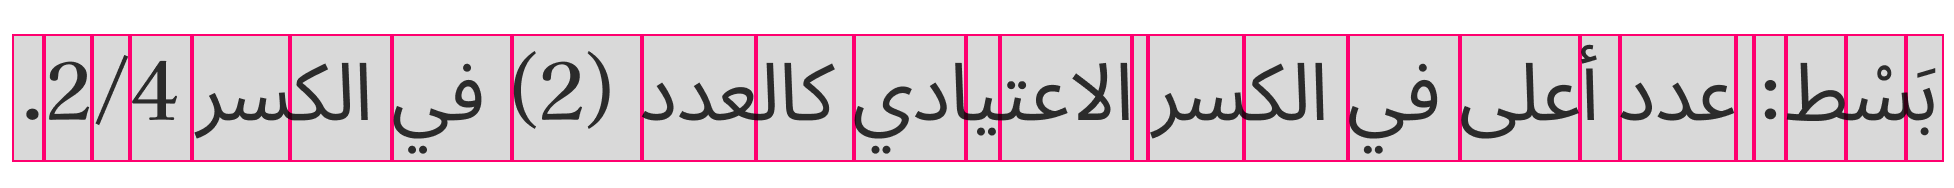
\includegraphics[width=0.6\textwidth]{tokenized-sentence.png}
    \caption{A sample sentence tokenized using the mT5 tokenizer}
    \label{fig:tokenized-sentence}
\end{figure}

\subsubsection{Model architecture}

The proposed model architecture leverages a pre-trained mT5 model as its foundation, particularly the encoder part of the model. The last hidden layer of the mT5 encoder contains the embedding information needed to represent the input sentence in the target words’ space. Figure \ref{fig:model-arch} illustrates the model architecture, which consists of an encoder, a pooling layer, and a linear layer.

The input is a vector of size 256, which is the tokenized and encoded input sentence. The input is then passed through the mT5 encoder, which outputs a matrix of shape (batch size, sequence length, hidden size). The last hidden state of the encoder is then passed through a pooling layer to transform it into a vector of a fixed length of 718. Finally, the output of the pooling layer is passed through a linear layer that transforms it into the desired target shape, which is 256 for electra, 768 for bertseg, and 768 for bertmsa.

\begin{figure}[H]
    \centering
    \captionsetup{justification=centering}
    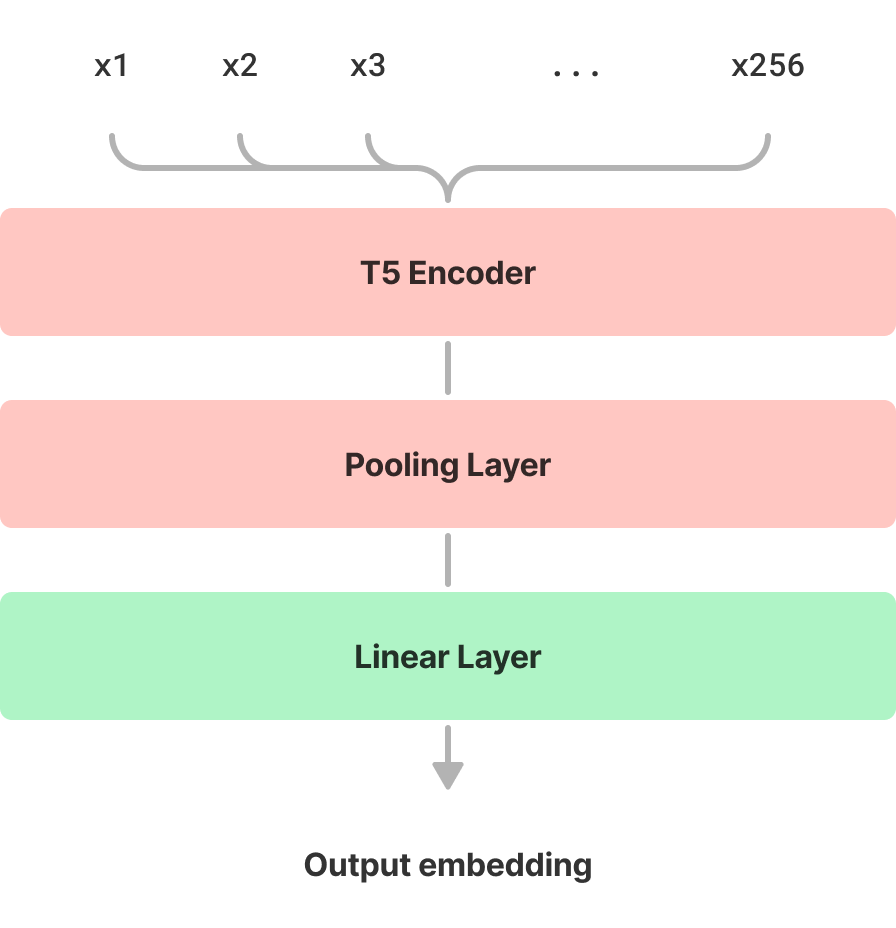
\includegraphics[width=0.6\textwidth]{model-arch.png}
    \caption{A sample sentence tokenized using the mT5 tokenizer}
    \label{fig:model-arch}
\end{figure}

The last hidden state of the mT5 encoder is not a vector, rather a matrix, and adapt it to output an embedding of a specific shape, a pooling layer will first transform the hidden state matrix to a vector of a fixed (the mT5 encoder output shape). This layer can be represented by the following equation. This equation calculates a weighted sum of the last hidden states \(O\) where the weights are determined by the attention mask \(A\), normalized by the total weight (or count of non-zero entries in \(A\) for each sequence).

\begin{equation}
    pool = \frac{\sum_{j,k} (O_{ijk} \cdot A_{ijk})}{\sum_j A_{ij}}
\end{equation}

The final layer is a linear layer that takes the output from the pooling layer, and transforms it into the desired target shape. The dataset includes three target embedding sizes: 256 for electra, 768 for bertseg, and 768 for bertmsa. To accommodate these distinct shapes, the final layer of the model is adapted with two variations based on the target size, resulting in three different models.

The task at hand is not a direct sequence to sequence problem, rather an information retrieval task. Therefore, the model's objective is to predict target word embeddings instead of the words themselves.

Finally, the pre-trained models employed for the encoder part are mT5 Base and AraT5 V2, both of which are variations of the T5 model. AraT5 V2 is a fine-tuned version of the mT5 base model on diverse Arabic data, making it more specialized for Arabic and suitable for our task \cite{Nagoudi2021}.

\newpage

\section{Data analysis and results}

\subsection{Environment setup}

This subsection details the software environment and hardware specifications used for example generation, model development, and experimentation. Primarily, the technical stack leverages Python and Google Colab for development.

For example generation, we utilized Postgres engine for SQL with the pgvector extension. This extension enables efficient storage and querying of vectors based on cosine similarity. Additionally, the HNSW (Hierarchical Navigable Small World) algorithm is used for indexing, facilitating fast and accurate nearest neighbor searches within the high-dimensional vector space.

Model development was conducted within a Google Colab environment equipped with a single A100 GPU and 12 GB RAM. The chosen framework for this task was PyTorch, which is specifically designed for deep learning. Additionally, few other libraries were employed, notably the Hugging Face Transformers for loading and training of pre-trained models with the transformer architecture.

\subsection{Data expansion analysis}

To generate an example for a single entry in the dataset, we first merge the word and its gloss. In Figure \ref{fig:examples-generation}, the word is \<بَسْط> and what comes after it is the gloss, which forms the input sentence. Next, the input is transformed into an embedding using the multilingual-22-12 model API, which results in a vector of size 768, this ensures we’re projecting the input into the Wikipedia dataset space. The next step is to find the closest texts to our input in the space, which is achievable using cosine similarity, such that the closest embedding to the input is the example we’re looking for.

\begin{figure}[H]
    \centering
    \captionsetup{justification=centering}
    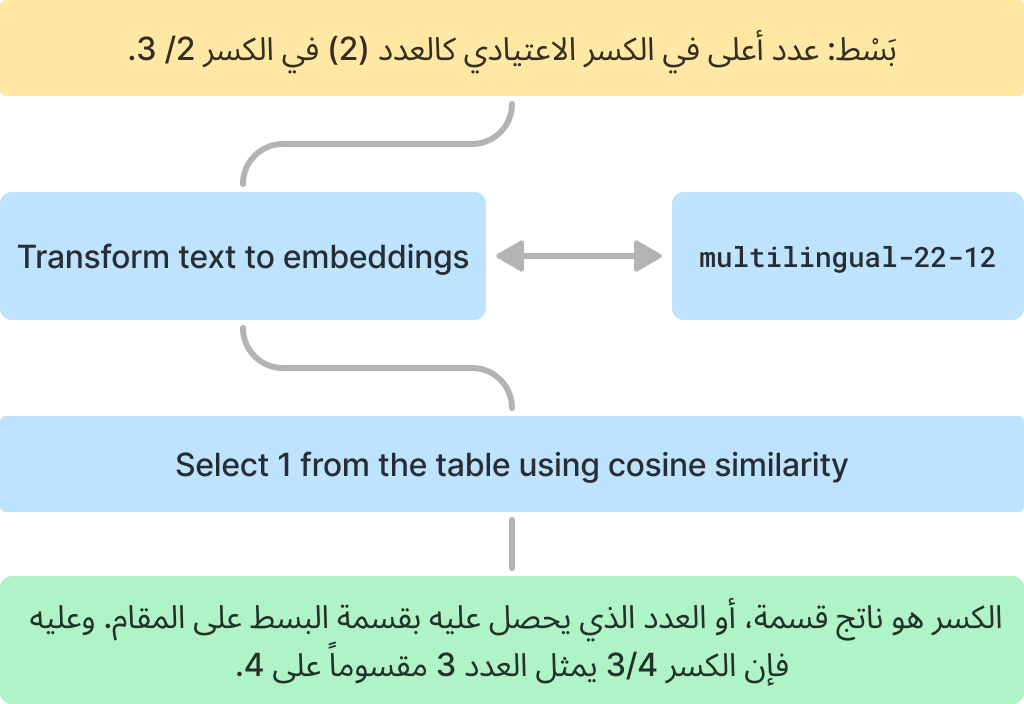
\includegraphics[width=0.6\textwidth]{examples-generation.png}
    \caption{The process of generating a single example for a word:gloss pair}
    \label{fig:examples-generation}
\end{figure}

While enriching the glosses with additional context demonstrates promise, it is not without limitations. Random sampling of the results reveals instances where the retrieved entries exhibit a weaker semantic connection to the dictionary entry. Consequently, human intervention remains necessary for data labeling and refinement to ensure better quality, potentially augmented by incorporating additional data sources to enrich the retrieval process.

\subsection{Training}

The training is done on the training set, with Mean Square Error loss function and an Adam optimizer with a learning rate value of 3e-5, which has been obtained via trial and error. Training has been done for 1 epoch, as with more epochs we noticed an overfitting over the training data, which is expected given that we’re only training a single linear layer. Figure \ref{fig:training} shows the full training pipeline with target variations.

The only difference between the models is the target size, which is 256 for electra, 768 for bertseg, and 768 for bertmsa. The model is trained on the training set and evaluated on the validation set using cosine similarity and Mean Squared Error (MSE) as evaluation metrics.

The only trainable layer in the model is the linear layer, which is responsible for transforming the output of the pooling layer into the desired target shape. The rest of the model is frozen, as it is pre-trained and does not require further training.

\begin{figure}
    \centering
    \captionsetup{justification=centering}
    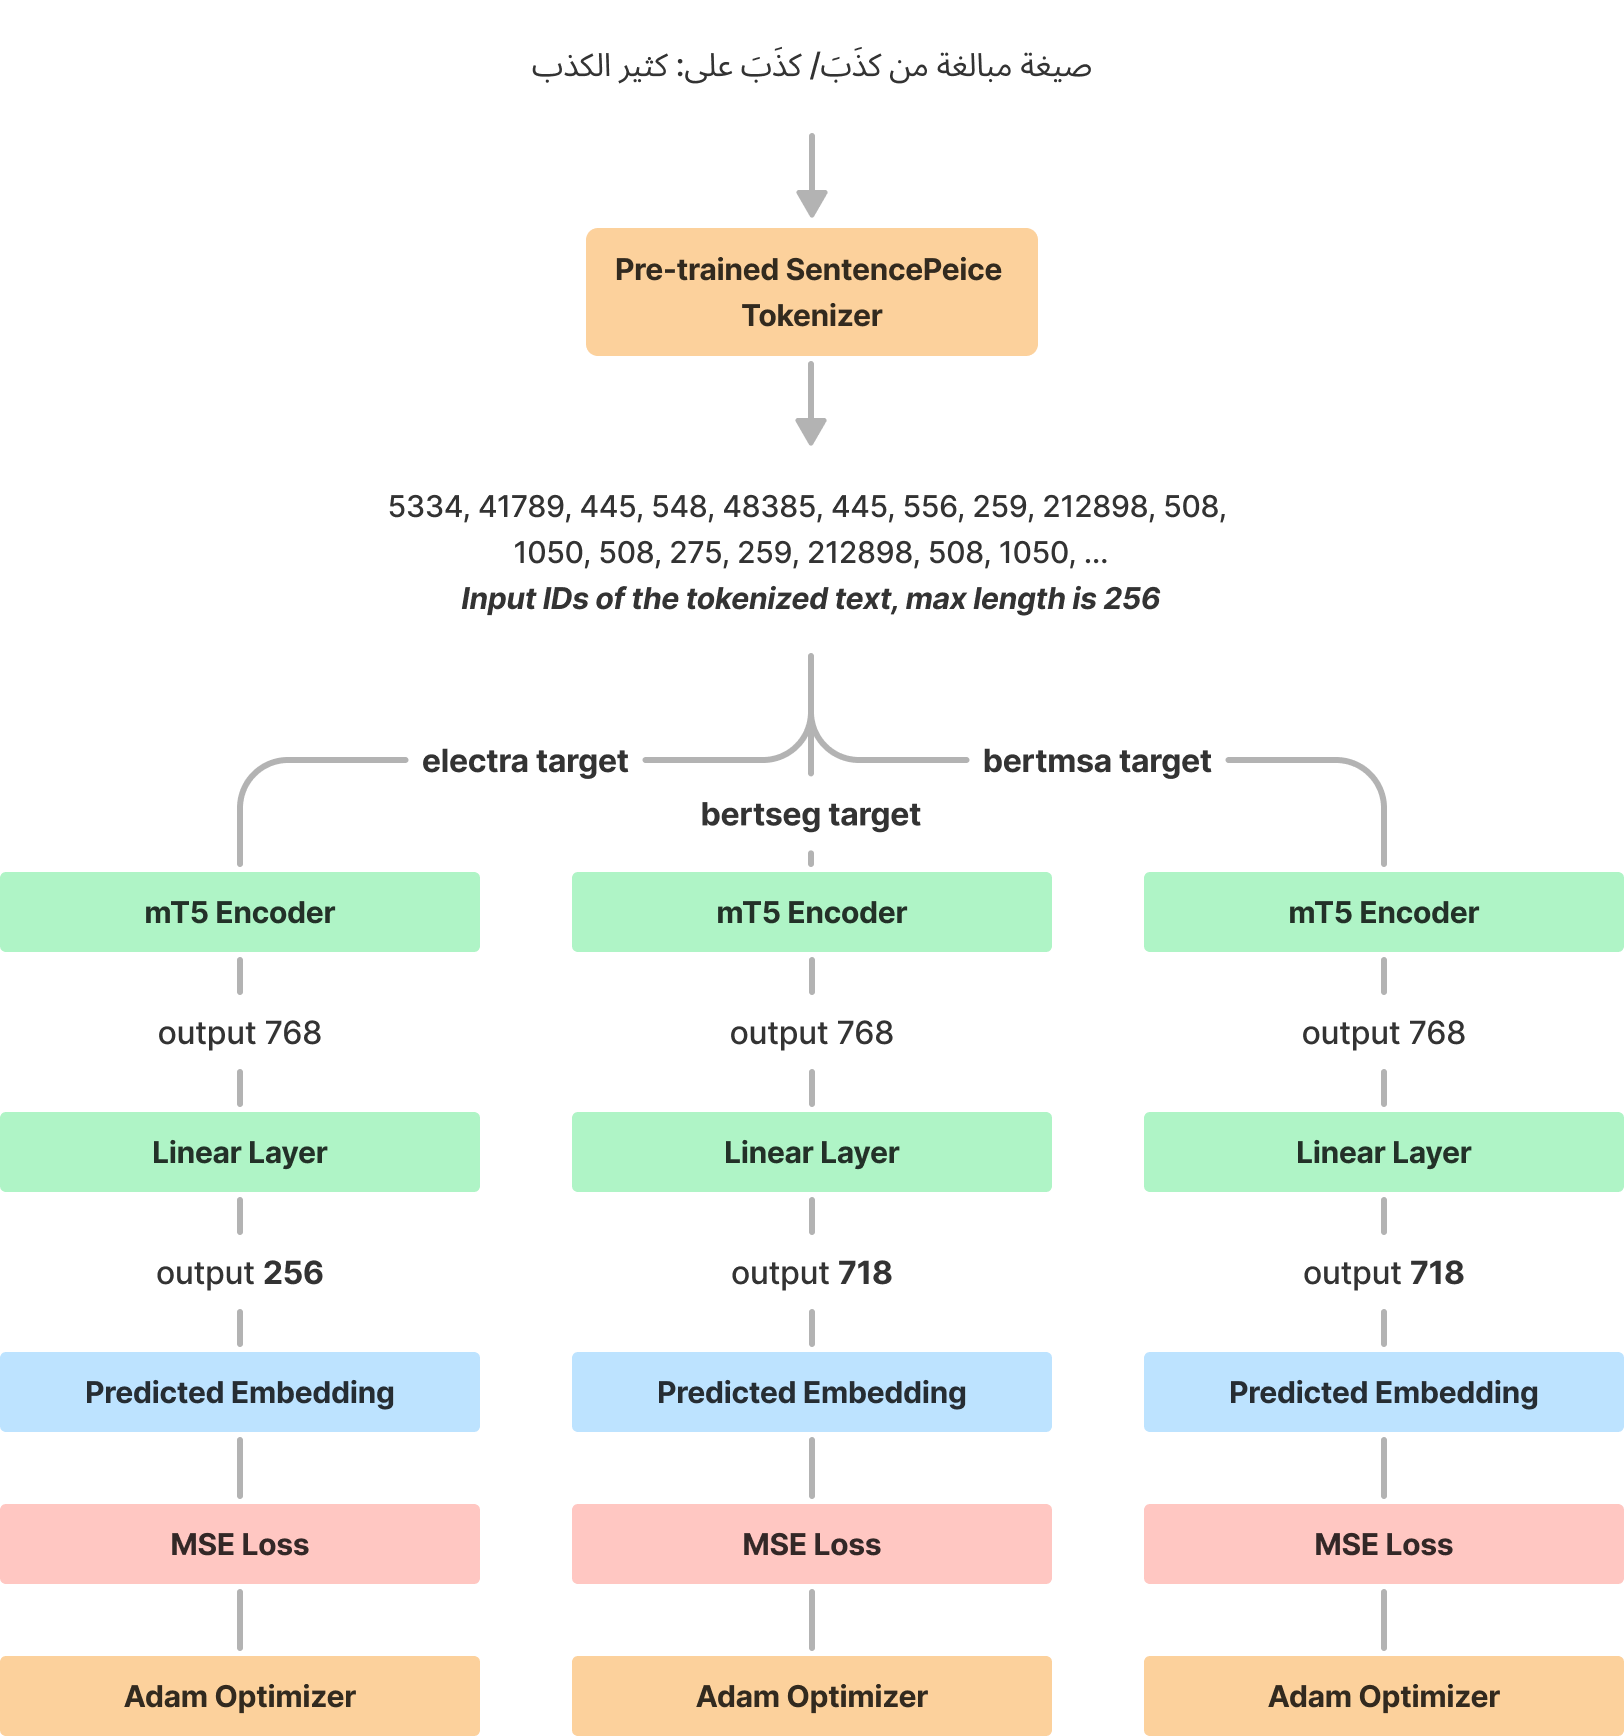
\includegraphics[width=\textwidth]{training.png}
    \caption{The training pipeline with target variations}
    \label{fig:training}
\end{figure}

\subsection{Evaluation results}

This subsection presents the final evaluation results of our model on the validation set. As the shared task withholds target values for the test set, its performance remains unevaluated. Once scores are submitted, official results will be announced alongside the winning solutions. Nonetheless, the validation set performance provides valuable insights into the model's potential.

Cosine similarity \ref{eq:cosine-similarity} and MSE \ref{eq:mse} are employed as evaluation metrics, measuring the semantic similarity between embeddings and the reconstruction error, respectively. Table \ref{table:results} summarizes the final results of our models compared to the baseline models.

% Cosine Similarity Equation
\begin{equation}\label{eq:cosine-similarity}
    Cosine Similarity = \frac{A \cdot B}{\|A\| \times \|B\|}
\end{equation}

% MSE Equation
\begin{equation}\label{eq:mse}
    MSE = \frac{1}{n} \sum_{i=1}^{n} (y_i - \hat{y_i})^2
\end{equation}

\begin{table}[H]
    \centering
    \caption{Results of the model on the validation set}
    \label{table:results}
    \renewcommand{\arraystretch}{1.5}%
    \begin{tabularx}{\textwidth}{|>{\raggedright}X|>{\raggedright\arraybackslash}X|X|X|}
        \hline
        \textbf{Model} & \textbf{Embedding} & \textbf{Cosine Similarity} & \textbf{MSE} \\
        \hline
        mT5-base (Ours) & electra & 0.5107 & 0.2498 \\\cline{2-4}
        & bertseg & 0.7657 & 0.0806 \\\cline{2-4}
        & bertmsa & 0.7012 & 0.3434 \\\cline{2-4}
        \hline
        AraT5v2-base (Ours) & electra & 0.5152 & 0.2459 \\\cline{2-4}
        & bertseg & 0.7656 & 0.0789 \\\cline{2-4}
        & bertmsa & 0.6965 & 0.3484 \\\cline{2-4}
        \hline
        CamelBERT (Baseline) & electra & 0.8185 & 0.2195 \\\cline{2-4}
        & bertseg & \textbf{0.8436*} & 0.0555 \\\cline{2-4}
        & bertmsa & 0.5113 & 0.2428 \\\cline{2-4}
        \hline
        MARBERT (Baseline) & electra & \textbf{0.6948*} & 0.5016 \\\cline{2-4}
        & bertseg & 0.7603 & 0.0818 \\\cline{2-4}
        & bertmsa & \textbf{0.7368*} & 0.1457 \\\cline{2-4}
        \hline
    \end{tabularx}
\end{table}

For cosine similarity, higher values (closer to 1) indicate better performance in capturing semantic relationships between the generated embeddings and the original word embedding. Lower MSE values indicate better reconstruction accuracy, meaning the model can more faithfully reproduce the original word embedding from the generated embeddings. The results presented are averages across the validation set.

Our mT5-base model trained on bertseg embeddings achieves the highest cosine similarity score (0.7657) among our models, marginally exceeding the MARBERT baseline (0.7603) by 0.0054. However, it falls short of the CamelBERT baseline across all embedding types, with the largest gap observed using electra embeddings (e.g. 0.8185 vs. 0.5107).

\begin{table}[H]
    \centering
    \caption{Predictions for a sample word:gloss pair}
    \label{table:results-sample}
    \renewcommand{\arraystretch}{1.5}%
    \begin{tabularx}{\textwidth}{|c|X|X|}
        \hline
        \textbf{Input} & \textbf{Top retrieved predictions} & \textbf{Ground truth} \\
        \hline
        \<منسوب إلى تاريخ، له أهمية كبيرة> & \<زراعي> & \<تاريخي> \\
        \hline
        \<جَرَّعَهُ الماءَ: سَقَاه إياه> & \<شِرْب> & \<جَرَّع> \\
        \hline
    \end{tabularx}
\end{table}

Table \ref{table:results-sample} showcases the model's predictions for two sample word:gloss pairs, highlighting the top retrieved predictions and the ground truth. It can be noticed that the model's predictions are not always accurate, with the first example predicting \<زراعي> instead of the correct \<تاريخي>, and the second example predicting \<شِرْب> instead of the correct \<جَرَّع>, though it can be seen that the predictions have some syntactic similarity to the ground truth, indicating that the model is learning some meaningful relationships between the words.

Possible explanations for the performance gap include the model's architecture, training duration, and the quality of the augmented examples. The mT5 model may require further fine-tuning or additional training epochs to achieve optimal performance. Moreover, the quality of the augmented examples may impact the model's ability to learn meaningful word embeddings, necessitating further refinement.

To further enhance the model's performance, we propose the following:
\begin{enumerate}
    \item \textbf{Hyperparameter Tuning:} Optimizing hyperparameters like learning rate, batch size, and optimizer settings could potentially improve performance.
    \item \textbf{Advanced Architectures:} Exploring more sophisticated architectures like larger pre-trained models (e.g., mT5-large) or incorporating techniques like selective training of specific model components could potentially lead to significant performance gains.
    \item \textbf{Fine-tuning:} Fine-tuning the model on a larger dataset or domain-specific data could improve its performance on the task by adapting the model to the specific characteristics of the data.
    \item \textbf{Transfer Learning:} Leveraging transfer learning from models pre-trained on similar tasks or domains could provide a head start for training the model on the reverse dictionary task.
    \item \textbf{Human Evaluation:} Conducting a human evaluation of the model's predictions to assess the quality of the generated word embeddings and identify areas where the model excels or falls short.
\end{enumerate} 

\newpage

\section{Conclusion}

This report presents a comprehensive overview of the Arabic Reverse Dictionary task, detailing the dataset, methodology, and results of our model. The proposed solution leverages a pre-trained mT5 model for word embedding retrieval, with the goal of surpassing the baseline performance on the cosine similarity metric. The model is trained on augmented examples generated from the Arabic Wikipedia dataset, aiming to enrich the glosses with additional context for improved performance.

The evaluation results on the validation set demonstrate the model's potential, with the mT5-base model trained on bertseg embeddings achieving the highest cosine similarity score among our models. However, the model falls short of the CamelBERT baseline across all embedding types, indicating room for improvement. Possible avenues for enhancing the model's performance include hyperparameter tuning, advanced architectures, fine-tuning, transfer learning, and human evaluation.

Despite the limitations, this domain is still of high importance in the field of Arabic NLP. Further research and experimentation are needed to address the challenges and limitations identified in this work, including a focus on data quality, model architecture, and evaluation metrics.

This work contributes to the growing body of research on Arabic reverse dictionaries, providing insights into the challenges and opportunities in this domain. By exploring novel approaches and methodologies, we aim to advance the state-of-the-art in Arabic reverse dictionary tasks and facilitate the development of more accurate and efficient word embedding retrieval systems.

\newpage

\printbibliography[title={References}]\label{lastpage}


\end{document}



